\documentclass[usenames,dvipsnames,tikz]{standalone}
\usetikzlibrary{patterns}
%\usepackage{amsmath,amssymb}
%\usepackage{xcolor}
\colorlet{tBlue}{RoyalBlue!35!Cerulean}
\colorlet{tRed}{Red}
\definecolor{tLightPink}{HTML}{FFD4EB} %tikz color
\definecolor{tLightOrange}{HTML}{FFE3B2}
\definecolor{tLightYellow}{HTML}{FFFBBD} %tikz color
\definecolor{tLightGreen}{HTML}{D3ECAA}
\definecolor{tDarkGreen}{HTML}{9BBF86} %tikz color %9BBF86
\definecolor{tTurquoise}{HTML}{ACFFEF} %tikz color %6FC4DD %7FE8F3
\definecolor{tLightBlue}{HTML}{CEF0FF} %tikz color %CEF0FF
\definecolor{tDarkBlue}{HTML}{95B5FF} %tikz color %95B5FF
\definecolor{tLightPurple}{HTML}{D8CFFD} %tikz color %ECDBFF
\definecolor{tPeach}{HTML}{F98F96} %tikz color %F98F96
\begin{document}
	
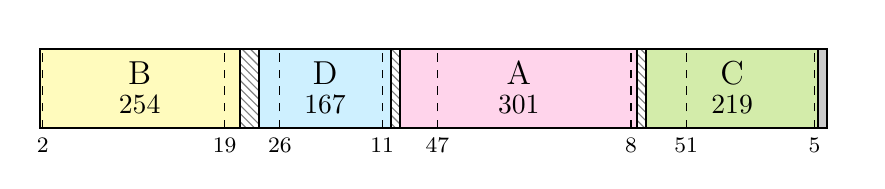
\begin{tikzpicture}
%\draw [help lines] (-1,-2) grid (11,5);
% 1=0.1, 2=0.15, 3=0.2, 4=0.25, 5=0.3
% 6 (3-27), 5 (8-42), 4 (33-65), 4 (16-22), 3 (13-28), 3 (11-40), 2 (35-50), 1 (15-30), 1 (14-38), 1 (4-57).

% ALTERNATIVE SCPP SINGLE BIN FEAS - ITEMS FIT INTO SINGLE BIN
\draw [thick, densely dashed, white] (10,-0.39) -- (10,1.26);
\draw [thick, white] (0,0) rectangle (10.37,1); %same size as infeas bin
\draw [thick] (0,0) rectangle (10,1); 

% B, D, A, C, 254, 167, 301, 219 (2-19, alpha=25, 26-11, alpha=12, 47-8, alpha=11, 51-5)
\path [fill=tLightYellow] (0,0) rectangle (2.54,1);
\path [fill=tLightBlue] (2.79,0) rectangle (4.46,1);
\path [fill=tLightPink] (4.58,0) rectangle (7.59,1);
\path [fill=tLightGreen] (7.7,0) rectangle (9.89,1);


\draw [thick] (2.54,0) -- (2.54,1);
\draw [thick] (2.79,0) -- (2.79,1);
\draw [thick] (4.46,0) -- (4.46,1);
\draw [thick] (4.58,0) -- (4.58,1);
\draw [thick] (7.59,0) -- (7.59,1);
\draw [thick] (7.7,0) -- (7.7,1);
\draw [thick] (9.89,0) -- (9.89,1);
\draw [thick, fill=black!20!white] (9.89,0) rectangle (10,1);

\draw [dashed] (0.04,0) -- (0.04,1); 
\draw [dashed] (2.35,0) -- (2.35,1);
\node at (1.27, 0.3) {$254$};
\node at (1.27, 0.7) {\large B};
\node [below] at (0.04,0) {\footnotesize{$2$}};
\node [below] at (2.35,0) {\footnotesize{$19$}};

%\draw [thick, fill=black!20!white] (2.54,0) rectangle (2.79,1);
\draw [thick, pattern = north west lines, pattern color=black!50!white] (2.54,0) rectangle (2.79,1); 

\draw [dashed] (3.05,0) -- (3.05,1);
\draw [dashed] (4.35,0) -- (4.35,1);
\node at (3.625, 0.3) {$167$};
\node at (3.625, 0.7) {\large D};
\node [below] at (3.05,0) {\footnotesize{$26$}};
\node [below] at (4.35,0) {\footnotesize{$11$}};

%\draw [thick, fill=black!20!white] (4.46,0) rectangle (4.58,1);
\draw [thick, pattern = north west lines, pattern color=black!50!white] (4.46,0) rectangle (4.58,1); 

\draw [dashed] (5.05,0) -- (5.05,1);
\draw [dashed] (7.51,0) -- (7.51,1);
\node at (6.085, 0.3) {$301$};
\node at (6.085, 0.7) {\large A};
\node [below] at (5.05,0) {\footnotesize{$47$}};
\node [below] at (7.51,0) {\footnotesize{$8$}};

%\draw [thick, fill=black!20!white] (7.59,0) rectangle (7.7,1);
\draw [thick, pattern = north west lines, pattern color=black!50!white] (7.59,0) rectangle (7.7,1); 

\draw [dashed] (8.21,0) -- (8.21,1);
\draw [dashed] (9.84,0) -- (9.84,1);
\node at (8.795, 0.3) {$219$};
\node at (8.795, 0.7) {\large C};
\node [below] at (8.21,0) {\footnotesize{$51$}};
\node [below] at (9.84,0) {\footnotesize{$5$}};


\draw [thick] (0,0) rectangle (10,1); 


\end{tikzpicture}

\end{document}